\subsection{Aeronautics \& Quaternions}
Aeronautics often deal with the problem of rotation.
An airplane has an ``internal frame", which needs to be corresponded to the `` body frame."
A common way to represent rotation on an airplane is with the following convention:
\begin{figure}[H]
\centering
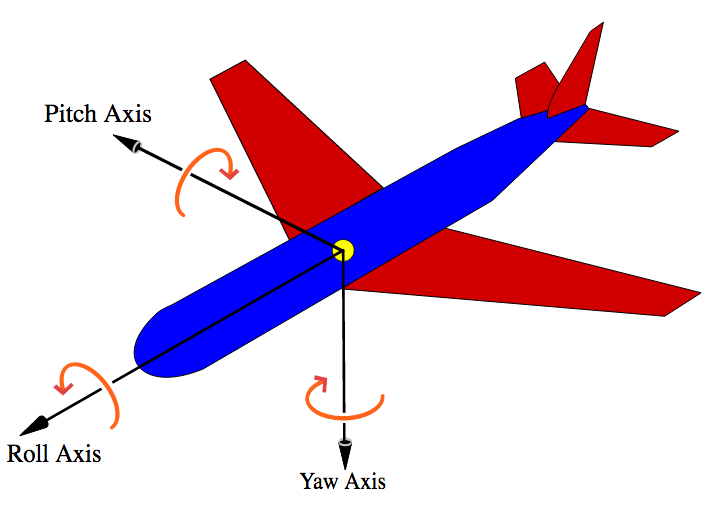
\includegraphics[width = .75\textwidth]{Figures/plane.png}
\caption{Roll, Pitch, and Yaw}
\label{fig:cycle}
\end{figure}
Roll, pitch, and yaw are simply Euler angles.
When flying a small plane, and rotating about a single axis, it may be easier to use Euler angles.
However, many large commerical airlines use computer assisted flight with many maneuvers done on autopilot.
Complicated rotations may be represented as an arbitrary rotation about an arbitrary axis, the perfect use case for quaternions.
There is another reason to use quaternions rather than rotation matrices when flying.
Rotations in 3D space can be thought of as a three gimbal system, where a gimbal is `` a pivoted support that allows the rotation of an object about a single axis.''
Figure \ref{fig:gimbal} shows an example of a 3-axis gimbal system.
\begin{figure}[H]
\centering
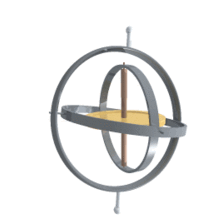
\includegraphics[width = .75\textwidth]{Figures/gimbal.png}
\caption{A 3-Axis Gimbal System}
\label{fig:gimbal}
\end{figure}
 This is essentially a visualization of Euler angles, where the deviation from the traditional 3-axis orientation can be used to keep track of the orientation of the system.
 Gimbals are commonly used in gyroscopes, aeronautics, and rocket systems.
 Gimbals in a 3-axis configuration have 3 degrees of freedom.
 A phenomenon can occur where gimbals end up in the same plane, and you lose a degree of freedom.
 Figure \ref{fig:gimlock} shows a locked gimbal system.

 \begin{figure}[H]
 \centering
 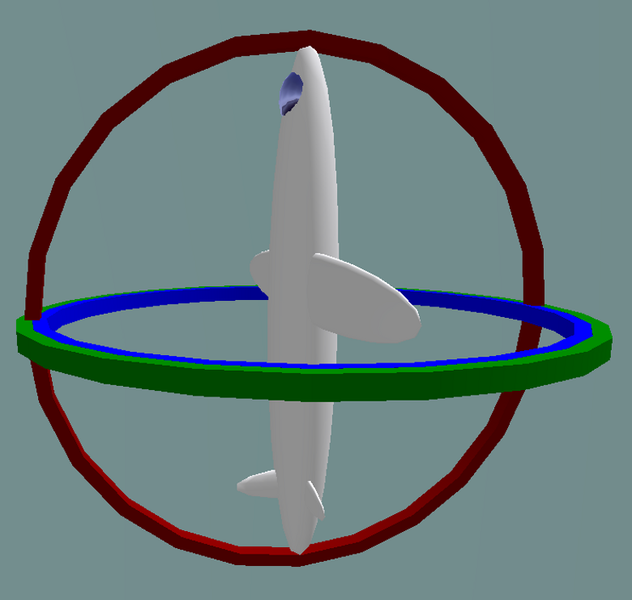
\includegraphics[width = .75\textwidth]{Figures/gimbal_lock.png}
 \caption{Roll and Yaw Gimbal Locked System}
 \label{fig:gimlock}
 \end{figure}

 In the above figure, the roll and yaw axes are now represented with a single gimbal.
 If the plane is told to rotate roll or yaw, the rotation is applied to the same axis.
 The only way to get out of gimbal lock is to rotate about the single gimbal.
 Gimbal lock is a property of Euler angles and rotation matrices.
 Here is the rotation matrix for the ($\alpha, \beta, \gamma$) angles that we did not calculate earlier.

 $$
 R =
 \begin{bmatrix}
 \text{cos }\beta \text{ cos }\gamma 																& -\text{sin }\gamma \text{ cos }\beta & \text{sin }\beta \\
 \text{sin }\beta \text{ cos }\alpha  \text{ cos }\gamma + \text{cos }\alpha \text{ sin }\gamma 	& - \text{sin }\gamma \text{ sin }\alpha \text{ sin }\beta + \text{cos }\alpha \text{ cos }\gamma & -\text{cos }\beta \text{ sin }\alpha \\
 -\text{sin }\beta \text{ cos }\gamma \text{ cos }\alpha + \text{sin }\alpha \text{ sin }\gamma 		& \text{sin }\gamma \text{ sin }\beta \text{ cos } \alpha + \text{ sin }\alpha \text{ cos } \gamma & \text{cos } \alpha \text{ cos } \beta
 \end{bmatrix}
 $$

Let us take $\beta= \frac{\pi}{2}$.
This results in the following rotation matrix:

$$
R =
\begin{bmatrix}
0 & 0 & 1 \\
\text{cos }\alpha  \text{ cos }\gamma + \text{cos }\alpha \text{ sin }\gamma 	& - \text{sin }\gamma \text{ sin }\alpha + \text{cos }\alpha \text{ cos }\gamma& 0 \\
 -\text{cos }\gamma \text{ cos }\alpha + \text{sin }\alpha \text{ sin }\gamma 		& \text{sin }\gamma \text{ cos } \alpha + \text{ sin }\alpha \text{ cos } \gamma  & 0
\end{bmatrix}
$$

Using trigonometric identities, we can simplify this rotation matrix as shown below.

$$
R =
\begin{bmatrix}
0 & 0 & 1 \\
\text{sin }(\alpha + \gamma) 	& \text{cos }(\alpha + \gamma) & 0 \\
-\text{cos }(\alpha + \gamma) 	& \text{sin }(\alpha + \gamma)   & 0
\end{bmatrix}
$$

Clearly, changing $\alpha$ or $\gamma$ has the same effect.
The gimbal is in effect, ``locked."
To fix this and get out of the gimbal lock, $\beta$ must be rotated first.
This is a problem inherant to Euler angles and their use in rotation matrices, but does not affect quaternions.

\subsection{Computer Graphics \& Quaternions}

Computer graphics, and specifically computer animation, rely on quaternions to express rotation between orientations.
Several game engines come with the ability to use quaternions on the back end.
The 2D and 3D cross-platform game engine called ``Unity", has instructions for coders and animators for implementing quaternions in their projects.
There are several reasons that quaternions offer advantages that have already been discussed, namely computation time, memory needed to represent a single rotation, and avoiding gimbal lock.
There is one other reason that quaternions offer an advantage to rotation matrices.
To investigate this, let us look at the basics of animation.
\subsubsection{Animation}
Animation relies on simulating three dimensional objects on a rigid frame and projecting them onto a 2D surface.
Tranformations (rotations and translations) are used to move objects between orientations and positions.
Methods such as spherical interpolation can be used to control the position of infinitely distant light sources, or to model features on a globe.
Let's say we are trying to animate a health bar in a video game.
We might pick several points that we want the bar to go through, and then perform a linear interpolation to fill in the points between.
It would not be too hard to pick some points that are evenly spaced apart, so that the movement does not appear to be jerky when rendered in an animation.
This method, shortened to \textit{lerp}, is commonly used for interpolating linear distance or velocity.
However, \textit{lerp} does not work well when trying to do spherical interpolation, shortened to \textit{slerp} \cite{animation}. 
\\ \\ Imagine we are trying to animate an object about an arbitrary axis, $\beta$, and by an arbitrary angle, $\theta$.
We have discussed several methods for obtaining the rotation about $\beta$ by $\theta$.
We could, for example, compute several different Euler angles and then individually rotate about each axis to achieve the desired rotation.
However, despite being valid mathematically, this would look pretty odd when animated.
Another solution might be to rotate using the quaternion, or rotation matrix, but linearly interpolated.
This is a natural rotation, but might appear jerky because the interpolation is not smooth, and if using a rotation matrix, we could still run into the problem of gimbal lock.
The solution is to use \textit{slerp} to animate a smooth interpolation with quaternions.
This achieves the desired smoothness, without fear of gimbal lock.
The mechanics behind \textit{slerp} are outside of the scope of this paper, but it works by keeping a constant speed.
The geometric formula for \textit{slerp}, as detailed by Ken Shoemaker, is given below in Equation \ref{eq:slerp}:

\begin{equation}
	Slerp(p_0, p_1, t) = \frac{sin[(1-t)\Omega]}{sin\Omega}p_0 + \frac{sin[t\Omega]}{sin\Omega}p_1
	\label{eq:slerp}
\end{equation}

When using Slerp to interpolate quaternions, it produces a uniform angular velocity around a rotation axis.
The same equation using quaternions is shown below in Equation \ref{eq:slerp2}:

\begin{equation}
	Slerp(q_0, q_1, t) = (q_1q_0^{-1})^tq_0
\label{eq:slerp2}
\end{equation}

To investigate the application of Slerp, we have written some MATLAB code to interpolate a vector rotation.
This code for this is shown below.

\begin{verbatim}
	%% Sean Turner
	%% University of Maine, Department of Mathematics and Statistics Capstone
	%% Spring 2017
	v = [1 .5 1]; % vector
	iterations = 100;
	p = [1 0 0 0]; % initial quaternion, does not rotate
	q = [1 0 1 0]; % Random Quaternion
	quat2eul(q) %Makes visualization easier, return euler angles in ZYX

	pn = quatnormalize(p); % normalization to unit quaternions
	qn = quatnormalize(q);
	qi = quatinterp(pn,qn,1/iterations,'slerp'); % performs interpolation between extremes

	plot3([0 v(1)], [0 v(2)], [0 v(3)]); % plot initial vector
	grid on;
	hold on;
	r = quatrotate(p,v); % doesn't rotate, but initializes r

	for i = 1:iterations % loops over iterations and applies rotation about quaternion
	    r = quatrotate(qi, r);
	    plot3([0 r(1)], [0 r(2)], [0 r(3)]);
	end

	rotate3d; % allows for click and drag in 3d plot
\end{verbatim}

Using an iteration value of 2 gives the following result.

\begin{figure}[H]
\centering
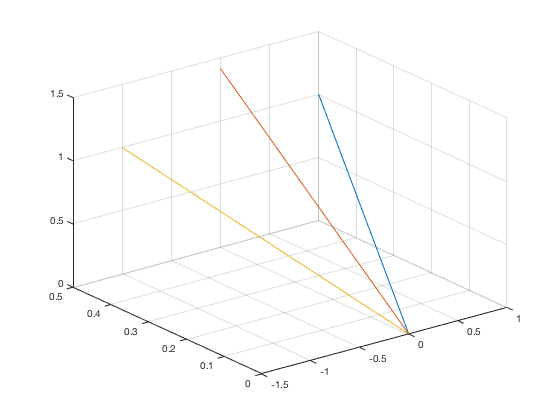
\includegraphics[width = .75\textwidth]{Figures/slerp2.png}
\caption{Slerp Example with 3 Iterations}
\label{fig:slerp3}
\end{figure}

The quaternion used in the code rotates the vector about the y-axis by an angle of $90^\circ$.
Notice the spherical interpolation of the second vector.
Using an iteration value of 100 yields Figure \ref{fig:slerp100}.


\begin{figure}[H]
\centering
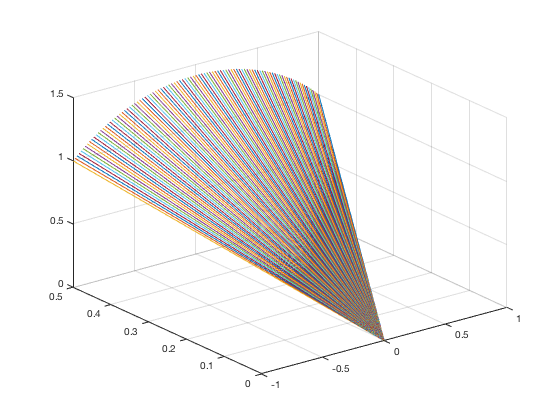
\includegraphics[width = .75\textwidth]{Figures/slerp100.png}
\caption{Slerp Example with 100 Iterations}
\label{fig:slerp100}
\end{figure}

Here the spherical interpolation is more clearly noticable.
The MATLAB code is easy to use, and performs the necessary interpolation quickly.
